%!TeX encoding = UTF-8
%!TeX program = xelatex
\documentclass[notheorems, aspectratio=54]{beamer}
% aspectratio: 1610, 149, 54, 43(default), 32

\usepackage{latexsym}
\usepackage{amsmath,amssymb}
\usepackage{mathtools}
\usepackage{color,xcolor}
\usepackage{graphicx}
\usepackage{algorithm}
\usepackage{amsthm}
\usepackage{graphicx}
\usepackage{subcaption}
\usepackage[export]{adjustbox}
\usepackage{wrapfig}
\usepackage{lmodern} % 解决 font warning
% \usepackage[UTF8]{ctex}
\usepackage{animate} % insert gif

\usepackage{lipsum} % To generate test text
\usepackage{ulem} % 下划线,波浪线

\usepackage{listings} % display code on slides; don't forget [fragile] option after \begin{frame}

% ----------------------------------------------
% tikx
\usepackage{framed}
\usepackage{tikz}
\usepackage{pgf}
\usetikzlibrary{calc,trees,positioning,arrows,chains,shapes.geometric,%
    decorations.pathreplacing,decorations.pathmorphing,shapes,%
    matrix,shapes.symbols}
\pgfmathsetseed{1} % To have predictable results
% Define a background layer, in which the parchment shape is drawn
\pgfdeclarelayer{background}
\pgfsetlayers{background,main}

% define styles for the normal border and the torn border
\tikzset{
  normal border/.style={black!70!gray, decorate,
     decoration={random steps, segment length=2.5cm, amplitude=.7mm}},
  torn border/.style={black!70!gray, decorate,
     decoration={random steps, segment length=.5cm, amplitude=1.7mm}}}

% Macro to draw the shape behind the text, when it fits completely in the
% page
\def\parchmentframe#1{
\tikz{
  \node[inner sep=2em] (A) {#1};  % Draw the text of the node
  \begin{pgfonlayer}{background}  % Draw the shape behind
  \fill[normal border]
        (A.south east) -- (A.south west) --
        (A.north west) -- (A.north east) -- cycle;
  \end{pgfonlayer}}}

% Macro to draw the shape, when the text will continue in next page
\def\parchmentframetop#1{
\tikz{
  \node[inner sep=2em] (A) {#1};    % Draw the text of the node
  \begin{pgfonlayer}{background}
  \fill[normal border]              % Draw the ``complete shape'' behind
        (A.south east) -- (A.south west) --
        (A.north west) -- (A.north east) -- cycle;
  \fill[torn border]                % Add the torn lower border
        ($(A.south east)-(0,.2)$) -- ($(A.south west)-(0,.2)$) --
        ($(A.south west)+(0,.2)$) -- ($(A.south east)+(0,.2)$) -- cycle;
  \end{pgfonlayer}}}

% Macro to draw the shape, when the text continues from previous page
\def\parchmentframebottom#1{
\tikz{
  \node[inner sep=2em] (A) {#1};   % Draw the text of the node
  \begin{pgfonlayer}{background}
  \fill[normal border]             % Draw the ``complete shape'' behind
        (A.south east) -- (A.south west) --
        (A.north west) -- (A.north east) -- cycle;
  \fill[torn border]               % Add the torn upper border
        ($(A.north east)-(0,.2)$) -- ($(A.north west)-(0,.2)$) --
        ($(A.north west)+(0,.2)$) -- ($(A.north east)+(0,.2)$) -- cycle;
  \end{pgfonlayer}}}

% Macro to draw the shape, when both the text continues from previous page
% and it will continue in next page
\def\parchmentframemiddle#1{
\tikz{
  \node[inner sep=2em] (A) {#1};   % Draw the text of the node
  \begin{pgfonlayer}{background}
  \fill[normal border]             % Draw the ``complete shape'' behind
        (A.south east) -- (A.south west) --
        (A.north west) -- (A.north east) -- cycle;
  \fill[torn border]               % Add the torn lower border
        ($(A.south east)-(0,.2)$) -- ($(A.south west)-(0,.2)$) --
        ($(A.south west)+(0,.2)$) -- ($(A.south east)+(0,.2)$) -- cycle;
  \fill[torn border]               % Add the torn upper border
        ($(A.north east)-(0,.2)$) -- ($(A.north west)-(0,.2)$) --
        ($(A.north west)+(0,.2)$) -- ($(A.north east)+(0,.2)$) -- cycle;
  \end{pgfonlayer}}}

% Define the environment which puts the frame
% In this case, the environment also accepts an argument with an optional
% title (which defaults to ``Example'', which is typeset in a box overlaid
% on the top border
\newenvironment{parchment}[1][Example]{%
  \def\FrameCommand{\parchmentframe}%
  \def\FirstFrameCommand{\parchmentframetop}%
  \def\LastFrameCommand{\parchmentframebottom}%
  \def\MidFrameCommand{\parchmentframemiddle}%
  \vskip\baselineskip
  \MakeFramed {\FrameRestore}
  \noindent\tikz\node[inner sep=1ex, draw=black!20, fill=black!90,
          anchor=west, overlay] at (0em, 2em) {\sffamily#1};\par}%
{\endMakeFramed}

% ----------------------------------------------

\mode<presentation>{
    \usetheme{Warsaw}
    % Boadilla CambridgeUS
    % default Antibes Berlin Copenhagen
    % Madrid Montpelier Ilmenau Malmoe
    % Berkeley Singapore Warsaw
    \usecolortheme{seagull}
    % beetle, beaver, orchid, whale, dolphin, seagull
    \useoutertheme{infolines}
    % infolines miniframes shadow sidebar smoothbars smoothtree split tree
    \useinnertheme{circles}
    % circles, rectangles, rounded, inmargin
}

% ---------------------------------------------------------------------
% Jet Black Theme
\setbeamercolor{normal text}{fg=white,bg=black!90}
\setbeamercolor{structure}{fg=white}

\setbeamercolor{alerted text}{fg=red!85!black}

\setbeamercolor{item projected}{use=item,fg=black,bg=item.fg!35}

\setbeamercolor*{palette primary}{use=structure,fg=structure.fg}
\setbeamercolor*{palette secondary}{use=structure,fg=structure.fg!95!black}
\setbeamercolor*{palette tertiary}{use=structure,fg=structure.fg!90!black}
\setbeamercolor*{palette quaternary}{use=structure,fg=structure.fg!95!black,bg=black!80}
\setbeamercolor*{framesubtitle}{fg=white}

\setbeamercolor*{block title}{parent=structure,bg=black!70!gray}
\setbeamercolor*{block body}{fg=black,bg=black!10}
\setbeamercolor*{block title alerted}{parent=alerted text,bg=black!15}
\setbeamercolor*{block title example}{parent=example text,bg=black!15}
% ---------------------------------------------------------------------


% ---------------------------------------------------------------------
% flow chart
\tikzset{
    >=stealth',
    punktchain/.style={
        rectangle,
        rounded corners,
        % fill=black!10,
        draw=white, very thick,
        text width=6em,
        minimum height=2em,
        text-centered,
        on chain
    },
    largepunktchain/.style={
        rectangle,
        rounded corners,
        draw=white, very thick,
        text width=10em,
        minimum height=2em,
        on chain
    },
    line/.style={draw, thick, <-},
    element/.style={
        tape,
        top color=white,
        bottom color=blue!50!black!60!,
        minimum width=6em,
        draw=blue!40!black!90, very thick,
        text width=6em,
        minimum height=2em,
        text-centered,
        on chain
    },
    every join/.style={->, thick,shorten >=1pt},
    decoration={brace},
    tuborg/.style={decorate},
    tubnode/.style={midway, right=2pt},
    font={\fontsize{10pt}{12}\selectfont},
}
% ---------------------------------------------------------------------

% code setting
\lstset{
    language=C++,
    basicstyle=\ttfamily\footnotesize,
    keywordstyle=\color{red},
    breaklines=true,
    xleftmargin=2em,
    numbers=left,
    numberstyle=\color[RGB]{222,155,81},
    frame=leftline,
    tabsize=4,
    breakatwhitespace=false,
    showspaces=false,
    showstringspaces=false,
    showtabs=false,
    morekeywords={Str, Num, List},
}

% ---------------------------------------------------------------------

\newcommand{\reditem}[1]{\setbeamercolor{item}{fg=red}\item #1}

% 缩放公式大小
\newcommand*{\Scale}[2][4]{\scalebox{#1}{\ensuremath{#2}}}

% 解决 font warning
\renewcommand\textbullet{\ensuremath{\bullet}}

% -------------------------------------------------------------

%% preamble
\title[Susskind Pipe Theory]{Susskind Pipe Theory}
% \subtitle{The subtitle}
\author{Behnam Lal Moghaddam}
\institute[Behnam Lal]{info@behnamlal.xyz}

% -------------------------------------------------------------

\begin{document}

% title frame
\begin{frame}
	\titlepage
\end{frame}

\begin{frame}
	\begin{center}
		\huge \textbf{Introduction}
	\end{center}
\end{frame}

% normal frame
\section{Susskind Pipe Theory}

\subsection{Introduction}
\begin{frame}
	\frametitle{Introduction}
	\begin{itemize}
		\item Leveraging the power of graph theory and Q-learning to optimize the flow of water in a network of pipes.
	\end{itemize}
\end{frame}

\subsection{Environment}
\begin{frame}
	\frametitle{Environment}
	\begin{itemize}
		\item Multiple input water sources
		\item Multiple output water sinks
		\item Junction nodes
		\item Pipes (have a chance to break, get clogged or increase capacity under pressure)
	\end{itemize}
	\begin{figure}
		\centering
		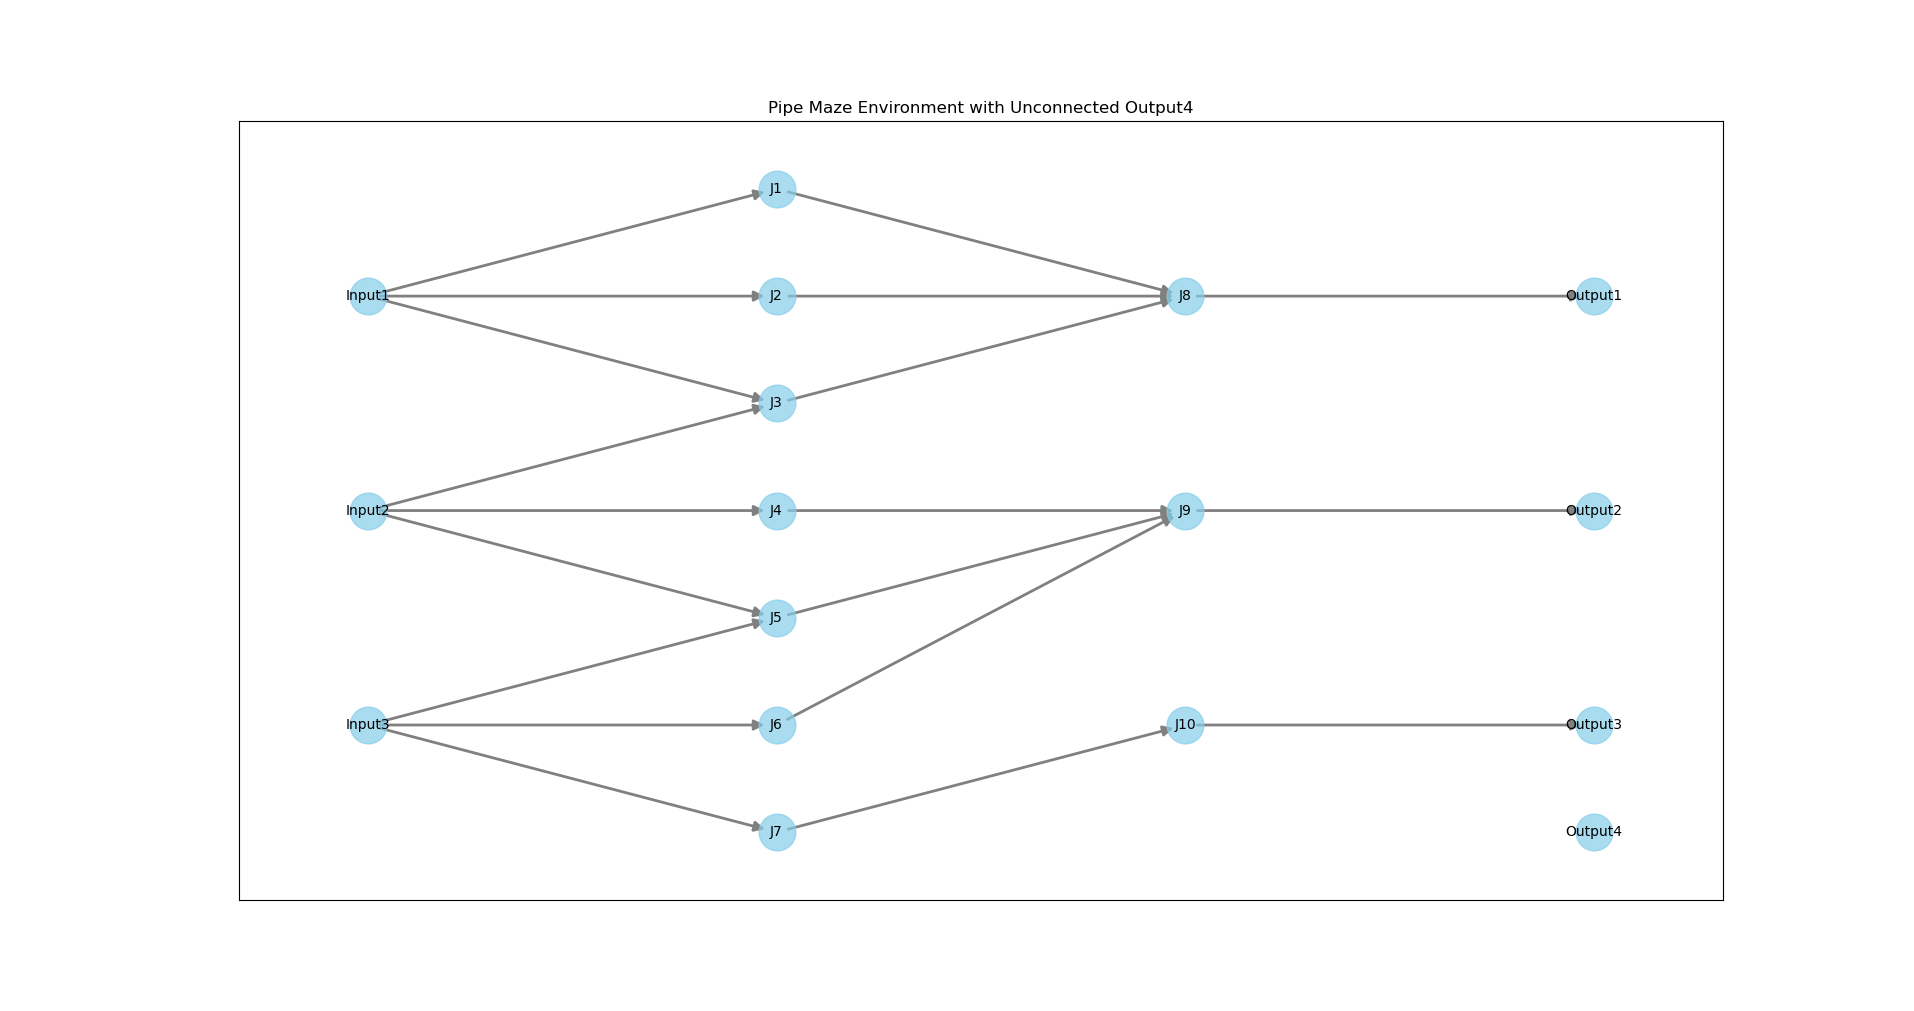
\includegraphics[width=0.8\textwidth]{fig-02.png}
		\caption{Pipe Network}
	\end{figure}
\end{frame}

\begin{frame}
	\frametitle{Algorithm}
	Currently used algorithms
	\begin{itemize}
		\item graph theory
		\item Q-learning
	\end{itemize}
	Other algorithms in consideration
	\begin{itemize}
		\item Monto Carlo
		\item integrate Fuzzy Rule Interpolation and use sparse fuzzy rule-bases to approximate the Q-function
		\item wire-fitted Neural Network Q-learning
	\end{itemize}
\end{frame}

\begin{frame}
	\frametitle{Problem Description}
	Maze Configuration
	\begin{itemize}
		\item Hidden layers of junction nodes between input and output
		\item Connection pipes have different characteristics: fixed capacity, adjustable capacity, potential for blockage or breakage.
	\end{itemize}
	Flow Dynamics
	\begin{itemize}
		\item Water divides at junction nodes based on downstream pipe capacity.
		\item Some pipe may increase capacity under pressure or may fail (break or clog)
		\item the output sinks have capacity. In case of extra water, It will overflow to next sink.
	\end{itemize}
\end{frame}

\begin{frame}
	\begin{center}
		\huge \textbf{The challenge is to find the optimal input sources for desired output amounts.}
	\end{center}
	\begin{itemize}
		\item It's possible that there exist no exact solution. A close answer is preferred.
	\end{itemize}
\end{frame}


\subsection{Implementation}
\begin{frame}
	\frametitle{Input}
	\begin{itemize}
		\item Maze Configuration:
		\begin{itemize}
			\item List of node IDs and their connections.
			\item Pipe characteristics and capacities.
		\end{itemize}
		\item Desired Water Output:
		\begin{itemize}
			\item Specified water amounts for output sinks.
		\end{itemize}
	\end{itemize}
\end{frame}


\begin{frame}
	\frametitle{Output}
	\begin{itemize}
		\item Optimal input sources and corresponding water pressures.
		\item Results can be printed or saved for further analysis.
	\end{itemize}
\end{frame}

\begin{frame}
	\frametitle{Class and Functions}
	\begin{itemize}
		\item Q-learning
		\item Reward function
		\item Exploration function
		\item Approximation function (planned)
		\item Environment class
		\item Pipe class
		\item Junction class
		\item Sink class
		\item input valve class
	\end{itemize}
\end{frame}

\begin{frame}
	\frametitle{Parameters}
	\begin{itemize}
		\item Learning rate = 0.1
		\item Discount factor = 0.5
		\item Exploration rate = 0.1
		\item Number of episodes = 1.0
	\end{itemize}
\end{frame}

\begin{frame}
	\frametitle{Simulation}
		amount of water in nodes, pipes and sinks are shown by color intensity.
\end{frame}


\begin{frame}
	\frametitle{Evaluation}
	\begin{itemize}
		\item Time taken to find the optimal policy.
		\item Accuracy of the policy in achieving the desired water distribution.
	\end{itemize}
\end{frame}

\begin{frame}
	\frametitle{Results}
	\begin{itemize}
		\item The algorithm is able to find the optimal policy in a reasonable amount of time.
		\item The policy is able to achieve the desired water distribution with high accuracy.
	\end{itemize}
\end{frame}

\begin{frame}
	\frametitle{Challenges I faced}
	\begin{itemize}
		\item The dynamic nature of the problem makes it difficult to find the optimal policy using traditional Q-learning.
	\end{itemize}
\end{frame}

\begin{frame}
	\frametitle{Extensions}
	\begin{itemize}
		\item Customizable nodes to adjust water pressure dynamically.
		\item Time constraints and priorities for output sinks.
		\item Consideration of water consumption rates over time.
	\end{itemize}
\end{frame}

\begin{frame}
	\frametitle{Relatable Problems}
	\begin{itemize}
		\item Design of computer networks.
		\item Circuit or chip connectivity.
		\item Understanding brain connectivity and potential applications in neural prosthetics.
	\end{itemize}
\end{frame}

% \begin{frame}
%     \begin{center}
%         \huge \textbf{Projects Overview}
%     \end{center}
% \end{frame}
%
% \begin{frame}
% 	\frametitle{Projects Overview}
% 	\centering \Large AI-powered drug discovery to aid pharmaceutical research
%     \vspace{20pt}
%     \begin{figure}\centering
%         \begin{minipage}{.5\textwidth}
%             \centering
%             \includegraphics[width=.6\linewidth]{src/drug_disc-01.jpg}
%             % \captionof{figure}{A figure}
%             \label{fig:test1}
%         \end{minipage}%
%         \begin{minipage}{.5\textwidth}
%             \centering
%             \includegraphics[width=.7\linewidth]{src/drug_disc-03.jpg}
%             % \captionof{figure}{Another figure}
%             \label{fig:test2}
%         \end{minipage}
%     \end{figure}
%
%
% \end{frame}
%
% \begin{frame}
% 	\frametitle{Projects Overview \tiny - AI-powered drug discovery to aid pharmaceutical research}
% 	\begin{itemize}
% 		\item Overview: The provision of a tool that can predict the effectiveness of a drug based on its chemical structure.
% 		\item Objective: limit the number of drugs that need to be tested in a lab.
% 		\item Technologies: chembl database, rdkit, LLM.
% 		\item Expected Impact: reduce the cost of drug discovery. (time and money)
% 		\item Marketing: pharmaceutical companies, research institutions, universities
% 	\end{itemize}
% \end{frame}
%
\begin{frame}
	\frametitle{Q\&A}
    \vspace{20pt}
    \begin{center}
        \huge \textbf{Any Questions?}
    \end{center}

\end{frame}

\begin{frame}
	% \frametitle{Closing Remarks}
    \vspace{20pt}
    \begin{center}
        \huge \textbf{Thank you for your time!}
    \end{center}

\end{frame}

% \begin{frame}
%     \frametitle{template for uml}
%
%     % Define block styles
%     \tikzset{
%         grayCircle/.style = {
%             draw,
%             circle,
%             node distance=2.5cm,
%             minimum size=1.5cm,
%             fill=black!20
%         }
%     }
%
%    \begin{figure}
%        \centering
%        \includegraphics[width=0.5\textwidth]{example-image} % Change "example-image" to the filename of your image
%        \caption{Caption for the image}
%        \label{fig:example}
%    \end{figure}
%
%     \center
%     \begin{tikzpicture}
%         \node[grayCircle] (age) {age};
%         \node[grayCircle, right of=age, style={fill=none}] (x) {x};
%         \node[grayCircle, right of=x, yshift=1.25cm] (t1) {test 1};
%         \node[grayCircle, below of=t1] (t2) {test 2};
%         \draw[->, >=latex] (age) -- (x);
%         \draw[->, >=latex] (x) -- (t1);
%         \draw[->, >=latex] (x) -- (t2);
%     \end{tikzpicture}
%
%     \begin{figure}
%         \caption{a template caption}
%     \end{figure}
%
% \end{frame}

\end{document}
